\documentclass[14pt,a4paper]{extarticle}

\usepackage[utf8]{inputenc}
\usepackage[T2A]{fontenc}
\usepackage[russian]{babel}
\usepackage{pscyr}

\usepackage{geometry}
\geometry{left=30mm,right=15mm,top=20mm,bottom=20mm}

\usepackage{setspace}
\singlespacing
\renewcommand{\baselinestretch}{1.0}
\setlength{\parskip}{0pt}

\usepackage{indentfirst}
\setlength{\parindent}{1.25cm}

\usepackage{amsmath,amssymb}
\usepackage{graphicx}
\usepackage{float}
\usepackage{caption}
\usepackage{enumitem}
\usepackage{booktabs}
\usepackage{tabularx}

\usepackage{titlesec}

\titleformat{\section}
  {\normalfont\fontsize{14}{18}\bfseries\filright}
  {\thesection}{1em}{}
\titlespacing*{\section}{1.25cm}{14pt}{14pt}

\titleformat{\subsection}
  {\normalfont\fontsize{14}{18}\bfseries\filright}
  {\thesubsection}{1em}{}
\titlespacing*{\subsection}{1.25cm}{14pt}{14pt}

\usepackage{tocloft}
\renewcommand{\cfttoctitlefont}{\hfill\fontsize{14}{18}\selectfont\bfseries}
\renewcommand{\cftaftertoctitle}{\hfill}
\renewcommand{\cftsecfont}{\normalfont}
\renewcommand{\cftsecpagefont}{\normalfont}
\renewcommand{\cftsubsecfont}{\normalfont}
\renewcommand{\cftsubsecpagefont}{\normalfont}
\renewcommand{\cftdotsep}{1}
\renewcommand{\cftsecleader}{\cftdotfill{\cftdotsep}}

\usepackage{listings}
\lstset{
  basicstyle=\ttfamily\small,
  frame=single,
  breaklines=true,
  showstringspaces=false,
  inputencoding=utf8,
  extendedchars=true,
  literate={а}{{\cyra}}1 {б}{{\cyrb}}1 {в}{{\cyrv}}1 {г}{{\cyrg}}1
           {д}{{\cyrd}}1 {е}{{\cyre}}1 {ж}{{\cyrzh}}1 {з}{{\cyrz}}1
           {и}{{\cyri}}1 {й}{{\cyrishrt}}1 {к}{{\cyrk}}1 {л}{{\cyrl}}1
           {м}{{\cyrm}}1 {н}{{\cyrn}}1 {о}{{\cyro}}1 {п}{{\cyrp}}1
           {р}{{\cyrr}}1 {с}{{\cyrs}}1 {т}{{\cyrt}}1 {у}{{\cyru}}1
           {ф}{{\cyrf}}1 {х}{{\cyrh}}1 {ц}{{\cyrc}}1 {ч}{{\cyrch}}1
           {ш}{{\cyrsh}}1 {щ}{{\cyrshch}}1 {ъ}{{\cyrhrdsn}}1 {ы}{{\cyrery}}1
           {ь}{{\cyrsftsn}}1 {э}{{\cyrerev}}1 {ю}{{\cyryu}}1 {я}{{\cyrya}}1
           {А}{{\CYRA}}1 {Б}{{\CYRB}}1 {В}{{\CYRV}}1 {Г}{{\CYRG}}1
           {Д}{{\CYRD}}1 {Е}{{\CYRE}}1 {Ж}{{\CYRZH}}1 {З}{{\CYRZ}}1
           {И}{{\CYRI}}1 {Й}{{\CYRISHRT}}1 {К}{{\CYRK}}1 {Л}{{\CYRL}}1
           {М}{{\CYRM}}1 {Н}{{\CYRN}}1 {О}{{\CYRO}}1 {П}{{\CYRP}}1
           {Р}{{\CYRR}}1 {С}{{\CYRS}}1 {Т}{{\CYRT}}1 {У}{{\CYRU}}1
           {Ф}{{\CYRF}}1 {Х}{{\CYRH}}1 {Ц}{{\CYRC}}1 {Ч}{{\CYRCH}}1
           {Ш}{{\CYRSH}}1 {Щ}{{\CYRSHCH}}1 {Ъ}{{\CYRHRDSN}}1 {Ы}{{\CYRERY}}1
           {Ь}{{\CYRSFTSN}}1 {Э}{{\CYREREV}}1 {Ю}{{\CYRYU}}1 {Я}{{\CYRYA}}1
           {ё}{{\cyryo}}1 {Ё}{{\CYRYO}}1,
  numbers=left,
  numberstyle=\tiny,
  tabsize=2,
  language=R
}

\usepackage{hyperref}
\hypersetup{
    colorlinks=true,
    linkcolor=black,
    urlcolor=blue,
    citecolor=black,
}

\usepackage{fancyhdr}
\pagestyle{fancy}
\fancyhf{}
\fancyfoot[R]{\thepage}
\renewcommand{\headrulewidth}{0pt}

\begin{document}

% =========================================================
% ТИТУЛЬНЫЙ ЛИСТ
% =========================================================
\thispagestyle{empty}
\begin{center}
МИНИСТЕРСТВО ОБРАЗОВАНИЯ РЕСПУБЛИКИ БЕЛАРУСЬ

\vspace{0.5em}

Учреждение образования

\textbf{<<Белорусский государственный университет\\информатики и радиоэлектроники>>}

\vspace{2em}

Факультет компьютерных систем и сетей

\vspace{0.5em}

Кафедра программного обеспечения информационных технологий
\end{center}

\vspace{4em}

\begin{center}
\textbf{ОТЧЁТ}

по лабораторной работе №1

\vspace{0.5em}

по дисциплине <<Стили и методы программирования>>

\vspace{1em}

\textbf{Тема: <<Знакомство с языком R>>}
\end{center}

\vspace{6em}

\begin{flushright}
\begin{minipage}{0.5\textwidth}
\textbf{Выполнил:}\\
Лебедевич Артем Владимирович\\
магистрант факультета\\
компьютерных систем и сетей\\
группы 556301

\vspace{1em}

\textbf{Преподаватель:}\\
Парамонов Антон Иванович\\
кандидат технических наук, доцент\\
заведующий кафедрой информационных\\
систем и технологий ИТТ БГУИР
\end{minipage}
\end{flushright}

\vfill

\begin{center}
Минск, 2026
\end{center}

\newpage

% =========================================================
% СОДЕРЖАНИЕ
% =========================================================
\tableofcontents
\newpage

% =========================================================
% ВВЕДЕНИЕ
% =========================================================
\addcontentsline{toc}{section}{Введение}
\section*{ВВЕДЕНИЕ}

Язык программирования R является одним из наиболее распространённых инструментов для статистического анализа данных и их визуализации. R предоставляет широкий набор встроенных функций для работы с векторами, матрицами, фреймами данных, а также обширную библиотеку графических средств.

Целью данной лабораторной работы является знакомство с языком R и средой разработки RStudio, освоение базовых конструкций языка: работа с векторами, матрицами и фреймами данных, а также построение графиков различных типов.

\newpage

% =========================================================
% РАЗДЕЛ 1
% =========================================================
\section{ОСОБЕННОСТИ УСТАНОВКИ R И IDE RSTUDIO}

Для выполнения лабораторной работы были установлены следующие программные средства:

1 Язык R~-- загружен с официального сайта The Comprehensive R Archive Network (CRAN) по адресу \url{https://cran.r-project.org/}. Для операционной системы macOS использован PKG-установщик. Установка выполнена в каталог по умолчанию.

2 Среда разработки RStudio~-- загружена с сайта \url{https://posit.co/downloads/}. Используется версия RStudio Desktop (бесплатная редакция). Установка на macOS осуществляется перетаскиванием приложения в папку Applications.

Особенности установки для macOS:
\begin{itemize}[nosep]
  \item необходимо сначала установить R, а затем RStudio, так как последняя использует интерпретатор R;
  \item при первом запуске macOS может запросить разрешение на открытие приложения от неидентифицированного разработчика;
  \item рекомендуется установить Xcode Command Line Tools для поддержки компиляции пакетов из исходного кода.
\end{itemize}

\newpage

% =========================================================
% РАЗДЕЛ 2
% =========================================================
\section{СОЗДАНИЕ И СОХРАНЕНИЕ ПРОЕКТА В RSTUDIO}

Для создания нового проекта в RStudio необходимо выполнить следующие действия:

1 Выбрать пункт меню \texttt{File -> New Project...}.

2 В открывшемся диалоге выбрать \texttt{New Directory -> New Project}.

3 Указать имя директории проекта и путь размещения.

4 Нажать кнопку \texttt{Create Project}.

Для сохранения скрипта используется сочетание клавиш \texttt{Cmd+S} (macOS) или \texttt{Ctrl+S} (Windows/Linux). Альтернативный вариант~-- пункт меню \texttt{File -> Save}.

Проект сохраняется автоматически в формате файла \texttt{.Rproj}, который содержит настройки рабочего окружения.

\newpage

% =========================================================
% РАЗДЕЛ 3
% =========================================================
\section{СПОСОБЫ ЗАПУСКА СКРИПТА НА ЯЗЫКЕ R}

Существует несколько способов запуска R-скрипта в среде RStudio:

1 \textbf{Запуск текущей строки или выделенного фрагмента.} Сочетание клавиш \texttt{Ctrl+Enter} (Windows) или \texttt{Cmd+Enter} (macOS). Выполняется только та строка, на которой стоит курсор, либо выделенный блок кода. Результат отображается в консоли. Этот способ удобен для пошаговой отладки.

2 \textbf{Запуск всего скрипта.} Сочетание клавиш \texttt{Ctrl+Shift+Enter} или кнопка \texttt{Source} на панели инструментов скрипта. Выполняется весь файл скрипта целиком.

3 \textbf{Запуск из консоли командой source().} В консоли вводится команда \texttt{source("имя\_скрипта.R")}. При этом скрипт выполняется целиком.

4 \textbf{Запуск из командной строки ОС.} Команда \texttt{Rscript имя\_скрипта.R} позволяет запустить скрипт без использования IDE.

Отличие способов заключается в объёме выполняемого кода и возможности пошаговой отладки. Первый способ наиболее удобен при разработке и отладке, второй и третий~-- при финальном запуске.

\newpage

% =========================================================
% РАЗДЕЛ 4
% =========================================================
\section{ФРАГМЕНТ КОДА ИНДИВИДУАЛЬНОГО ЗАДАНИЯ}

Ниже приведён полный код скрипта, реализующего все пункты индивидуального задания.

\begin{lstlisting}[caption={Скрипт lab1\_script.R}, label=lst:lab1]
# --- 1) Вектор чисел (успеваемость 8 студентов) ---
data1 <- c(8, 5, 9, 7, 3, 10, 6, 4)

# --- 3) Имена для значений вектора ---
names(data1) <- c("Иванов", "Петров", "Сидоров", "Козлов",
                   "Новиков", "Фёдоров", "Морозов", "Волков")

# --- 4) Столбиковая диаграмма ---
barplot(data1,
        main = "Успеваемость студентов",
        col = rainbow(length(data1)),
        ylab = "Оценка",
        las = 2, cex.names = 0.8)

# --- 5) Набор строковых переменных ---
data2 <- c("Алексей", "Борис", "Виктор", "Григорий",
            "Дмитрий", "Евгений", "Жан", "Захар")

# --- 6) Диаграмма с легендой и сортировкой ---
sorted_data1 <- sort(data1, decreasing = TRUE)
sorted_data2 <- data2[order(data1, decreasing = TRUE)]
barplot(sorted_data1,
        main = "Успеваемость (по убыванию)",
        col = rainbow(length(sorted_data1)),
        ylab = "Оценка", las = 2, cex.names = 0.8)
legend("topright", legend = sorted_data2,
       fill = rainbow(length(sorted_data2)),
       cex = 0.7, title = "Студенты")

# --- 7) Матрица A размерностью 4x5 ---
A <- matrix(c(2,5,8,1, 3,7,4,6, 9,2,5,3,
              1,8,6,4, 7,3,2,9),
            nrow = 4, ncol = 5)
colnames(A) <- paste("Предмет", 1:5)
rownames(A) <- paste("Группа", 1:4)

# --- 8) Мозаичная диаграмма ---
mosaicplot(A,
           main = "Мозаичная диаграмма матрицы A",
           color = heat.colors(ncol(A)), las = 1)

# --- 9) Фрейм данных ---
df <- data.frame(Имя = data2,
                 Оценка = as.numeric(data1))
print(df)

# --- 10) Итоговая информация ---
summary(df)
\end{lstlisting}

\newpage

% =========================================================
% РАЗДЕЛ 5
% =========================================================
\section{РЕЗУЛЬТАТЫ РАБОТЫ КОДА}

В данном разделе приведены экранные формы, отображающие результаты пошагового выполнения кода.

\begin{figure}[H]
  \centering
  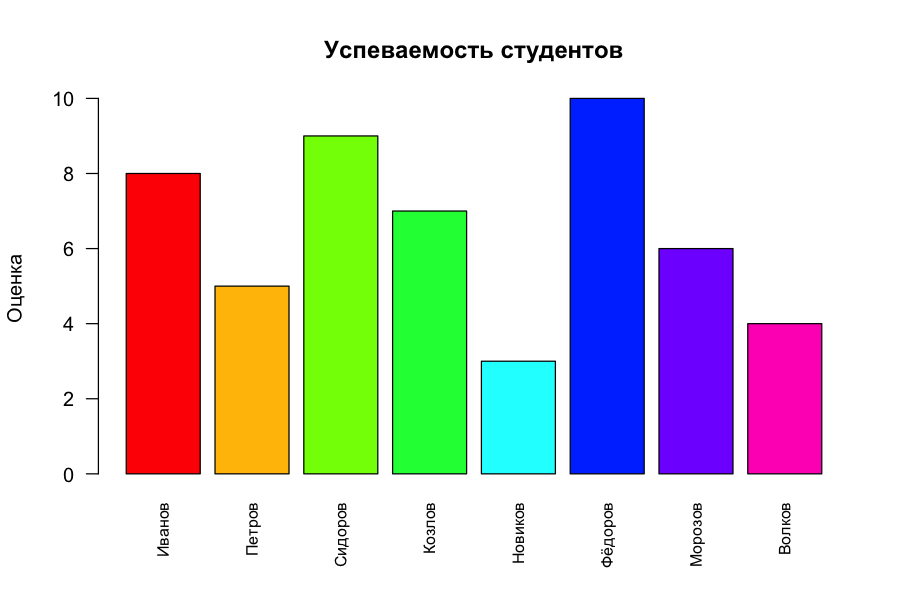
\includegraphics[width=0.85\textwidth]{screenshot1.png}
  \caption{Столбиковая диаграмма успеваемости студентов}
  \label{fig:barplot1}
\end{figure}

\begin{figure}[H]
  \centering
  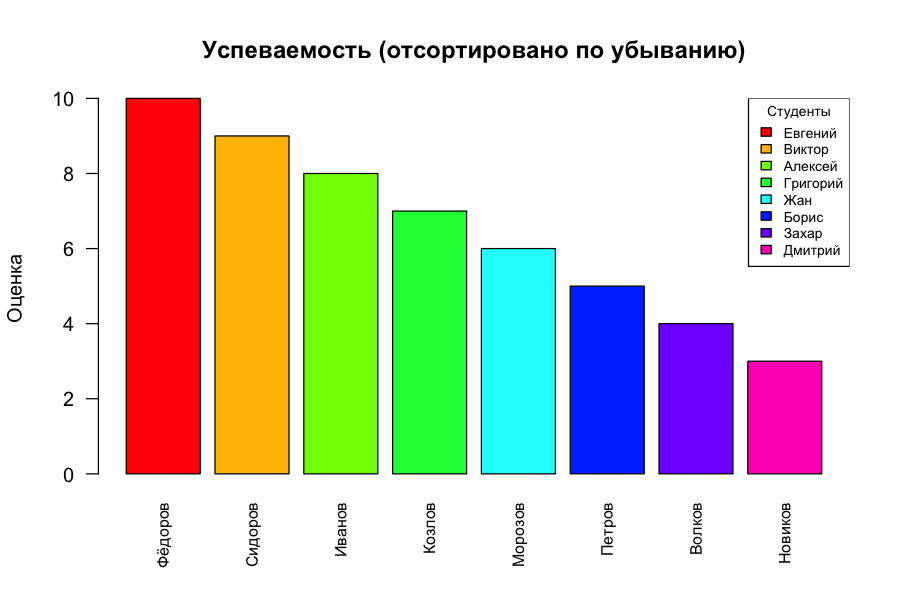
\includegraphics[width=0.85\textwidth]{screenshot2.png}
  \caption{Столбиковая диаграмма с легендой (отсортировано по убыванию)}
  \label{fig:barplot2}
\end{figure}

\begin{figure}[H]
  \centering
  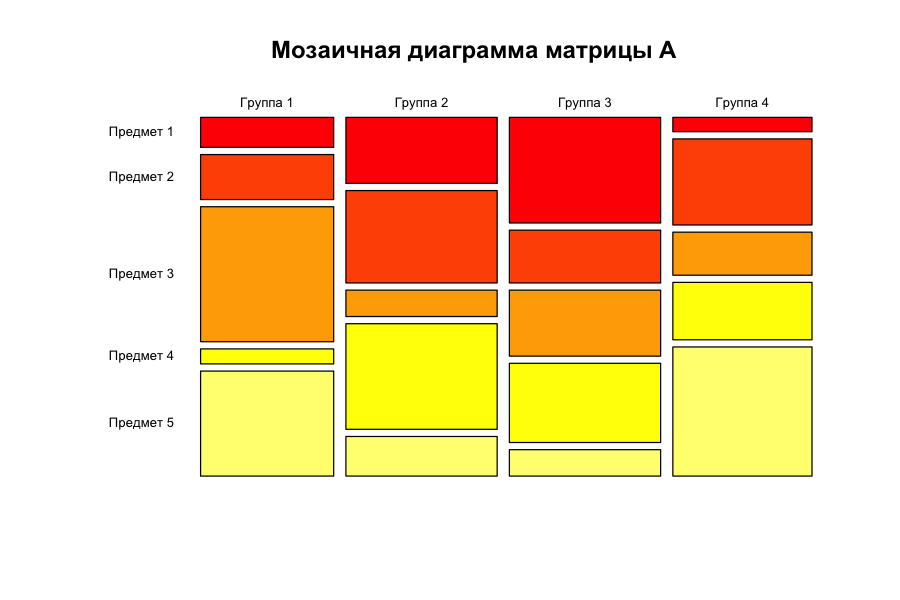
\includegraphics[width=0.85\textwidth]{screenshot3.png}
  \caption{Мозаичная диаграмма матрицы A}
  \label{fig:mosaic}
\end{figure}

\begin{figure}[H]
  \centering
  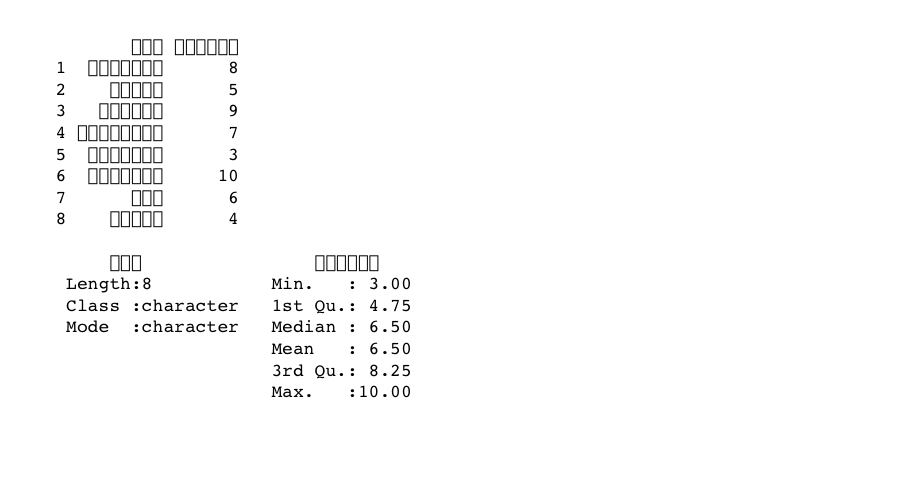
\includegraphics[width=0.85\textwidth]{screenshot4.png}
  \caption{Вывод фрейма данных и summary}
  \label{fig:summary}
\end{figure}

\newpage

% =========================================================
% ЗАКЛЮЧЕНИЕ
% =========================================================
\addcontentsline{toc}{section}{Заключение}
\section*{ЗАКЛЮЧЕНИЕ}

В ходе выполнения лабораторной работы были получены следующие результаты:

1 Установлены и настроены дистрибутив языка R и среда разработки RStudio на операционной системе macOS.

2 Изучены основные способы создания и сохранения проектов в RStudio, а также различные методы запуска R-скриптов.

3 Освоены базовые конструкции языка R: создание и именование векторов, работа с матрицами и фреймами данных.

4 Построены столбиковые и мозаичные диаграммы с использованием встроенных функций \texttt{barplot()} и \texttt{mosaicplot()}.

5 Изучены функции сортировки данных (\texttt{sort()}, \texttt{order()}) и получения описательной статистики (\texttt{summary()}).

\newpage

% =========================================================
% СПИСОК ИСПОЛЬЗОВАННЫХ ИСТОЧНИКОВ
% =========================================================
\addcontentsline{toc}{section}{Список использованных источников}
\section*{СПИСОК ИСПОЛЬЗОВАННЫХ ИСТОЧНИКОВ}

\begin{enumerate}[label=\arabic*,leftmargin=1.25cm]
  \item The Comprehensive R Archive Network [Электронный ресурс].~-- Режим доступа: \url{https://cran.r-project.org/}.~-- Дата доступа: 10.04.2026.
  \item RStudio project [Электронный ресурс].~-- Режим доступа: \url{https://www.rstudio.com/products/rstudio/}.~-- Дата доступа: 10.04.2026.
  \item RStudio IDE User Guide [Электронный ресурс].~-- Режим доступа: \url{https://docs.posit.co/ide/user/}.~-- Дата доступа: 10.04.2026.
  \item Шипунов, А.\,Б. Анализ данных с R / А.\,Б.~Шипунов, А.\,И.~Коробейников, Е.\,М.~Балдин [Электронный ресурс].~-- Режим доступа: \url{https://inp.nsk.su/~baldin/DataAnalysis/R/R-07-datamining.pdf}.~-- Дата доступа: 10.04.2026.
  \item Peng,~R.\,D. Mastering Software Development in R / R.\,D.~Peng, S.~Kross, B.~Anderson [Электронный ресурс].~-- Режим доступа: \url{https://bookdown.org/rdpeng/RProgDA/}.~-- Дата доступа: 10.04.2026.
\end{enumerate}

\end{document}
